\subsection{Components}

Figure \ref{fig:comp_dia} shows a high level view of the logical layout of the components in the MDApp.

\begin{figure}[H]
    \centering
    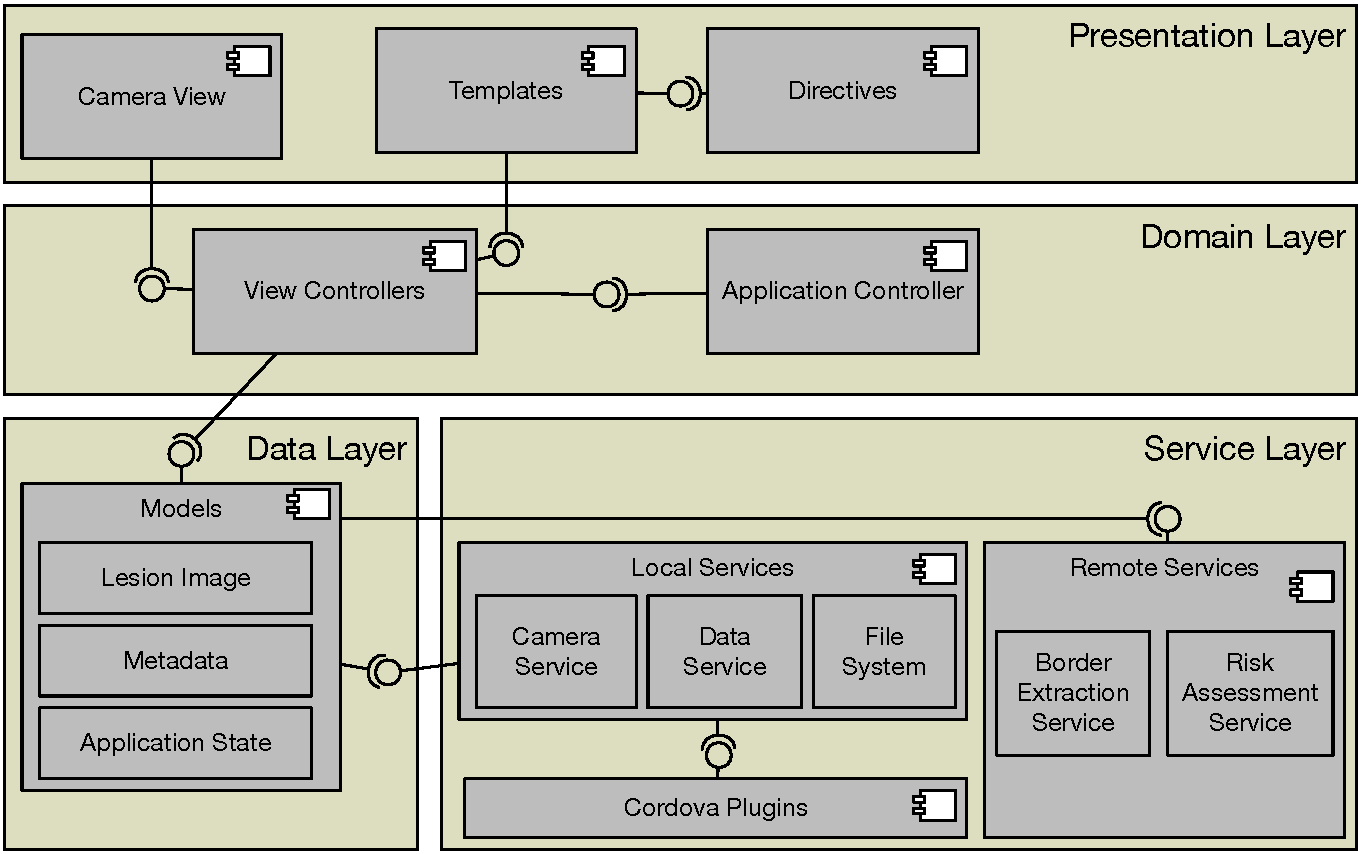
\includegraphics[width=\textwidth,keepaspectratio]{assets/architecture/compontent_diagram.pdf}
    \caption{Component diagram of the MDApp}
    \label{fig:comp_dia}
\end{figure}

\subsubsection{View Controllers}

Each view controller class is responsible for a specific view or partial view of the MDApp. In larger applications there might be multiple view controllers per “page” in a nested hierarchy. The MDApp will only require one controller per page, these are the HomeController, CameraController, AnalysisController and the ArchiveController. Each controller is responsible for preparing the data that will be displayed in the view as well as capturing and processing user events.

\subsubsection{Application Controller}
The application controller is a global controller that can manage the state of the app. It makes sure that the state is persevered when the MDApp is closed and restarted. It can also switch the user automatically from one view to another when appropriate or enable or disable the user interface when some activity is in progress.

\subsubsection{Templates, Directives and Camera View}
Except for the the Camera View all of the pages are created from HTML files that have prepared placeholders called directives. Directives are special markers in the HTML that the Angular framework uses to inject data and specific behaviour into the HTML element. Directives bundle together often used patterns into easily configurable markers that can be embedded into an HTML file.

The Camera View is an exception in the MDApp. The CameraView is an HTML template that overlays a realtime preview of the camera’s input. The realtime preview is not part of the Cordova/Phonegap browser view, it is a platform native view element that is provided by a 3rd party plugin. The cordova-plugin-camera-preview is a crossplatofrm wrapper around native code that allows the browser based javascript to communicate and control the camera preview view.

\subsubsection{Models}
The Models are relatively simple data classes. The MDApp does not require much buisiness logic for the data. The Models encapsulate some communication with some of the services so that the controllers can remain as simple as possible.

\subsubsection{Local Services}
The local services classes are just wrappers around the Cordova plugins. Cordova plugins offer a "raw" javascript api, the service classes will hide some of the complexity by making only the relevant functions available to the MDApp.

\subsubsection{Remote Services}
The remote services leverage the angular \$resource factory which provides easily configurable RESTful communication to online servers.

\subsubsection{Cordova Plugins}

In a hybrid architecture most of the logic is programmed in javascript, just like a normal web page. Communication with native system components and hardware APIs that a normal browser based environment does not have access can be enabled through plugins. Ideally these plugins unify the native APIs across all platforms. The MDApp uses the following cordova plugins:

   \paragraph{cordova-plugin-camera-preview}
   \paragraph{cordova-plugin-file-transfer}
   \paragraph{Cordova-sqlite-storage}

\subsection{Classes}

The class diagram in figure \ref{fig:class_dia} shows the structure and connections between the main classes of the MDApp. The service layer classes are singletons that encapsulate the functionality of some plugin into an easy to manage form. Static class level methods and attributes are underlined. The other methods and attributes have object level scope.

\begin{figure}[H]
    \centering
    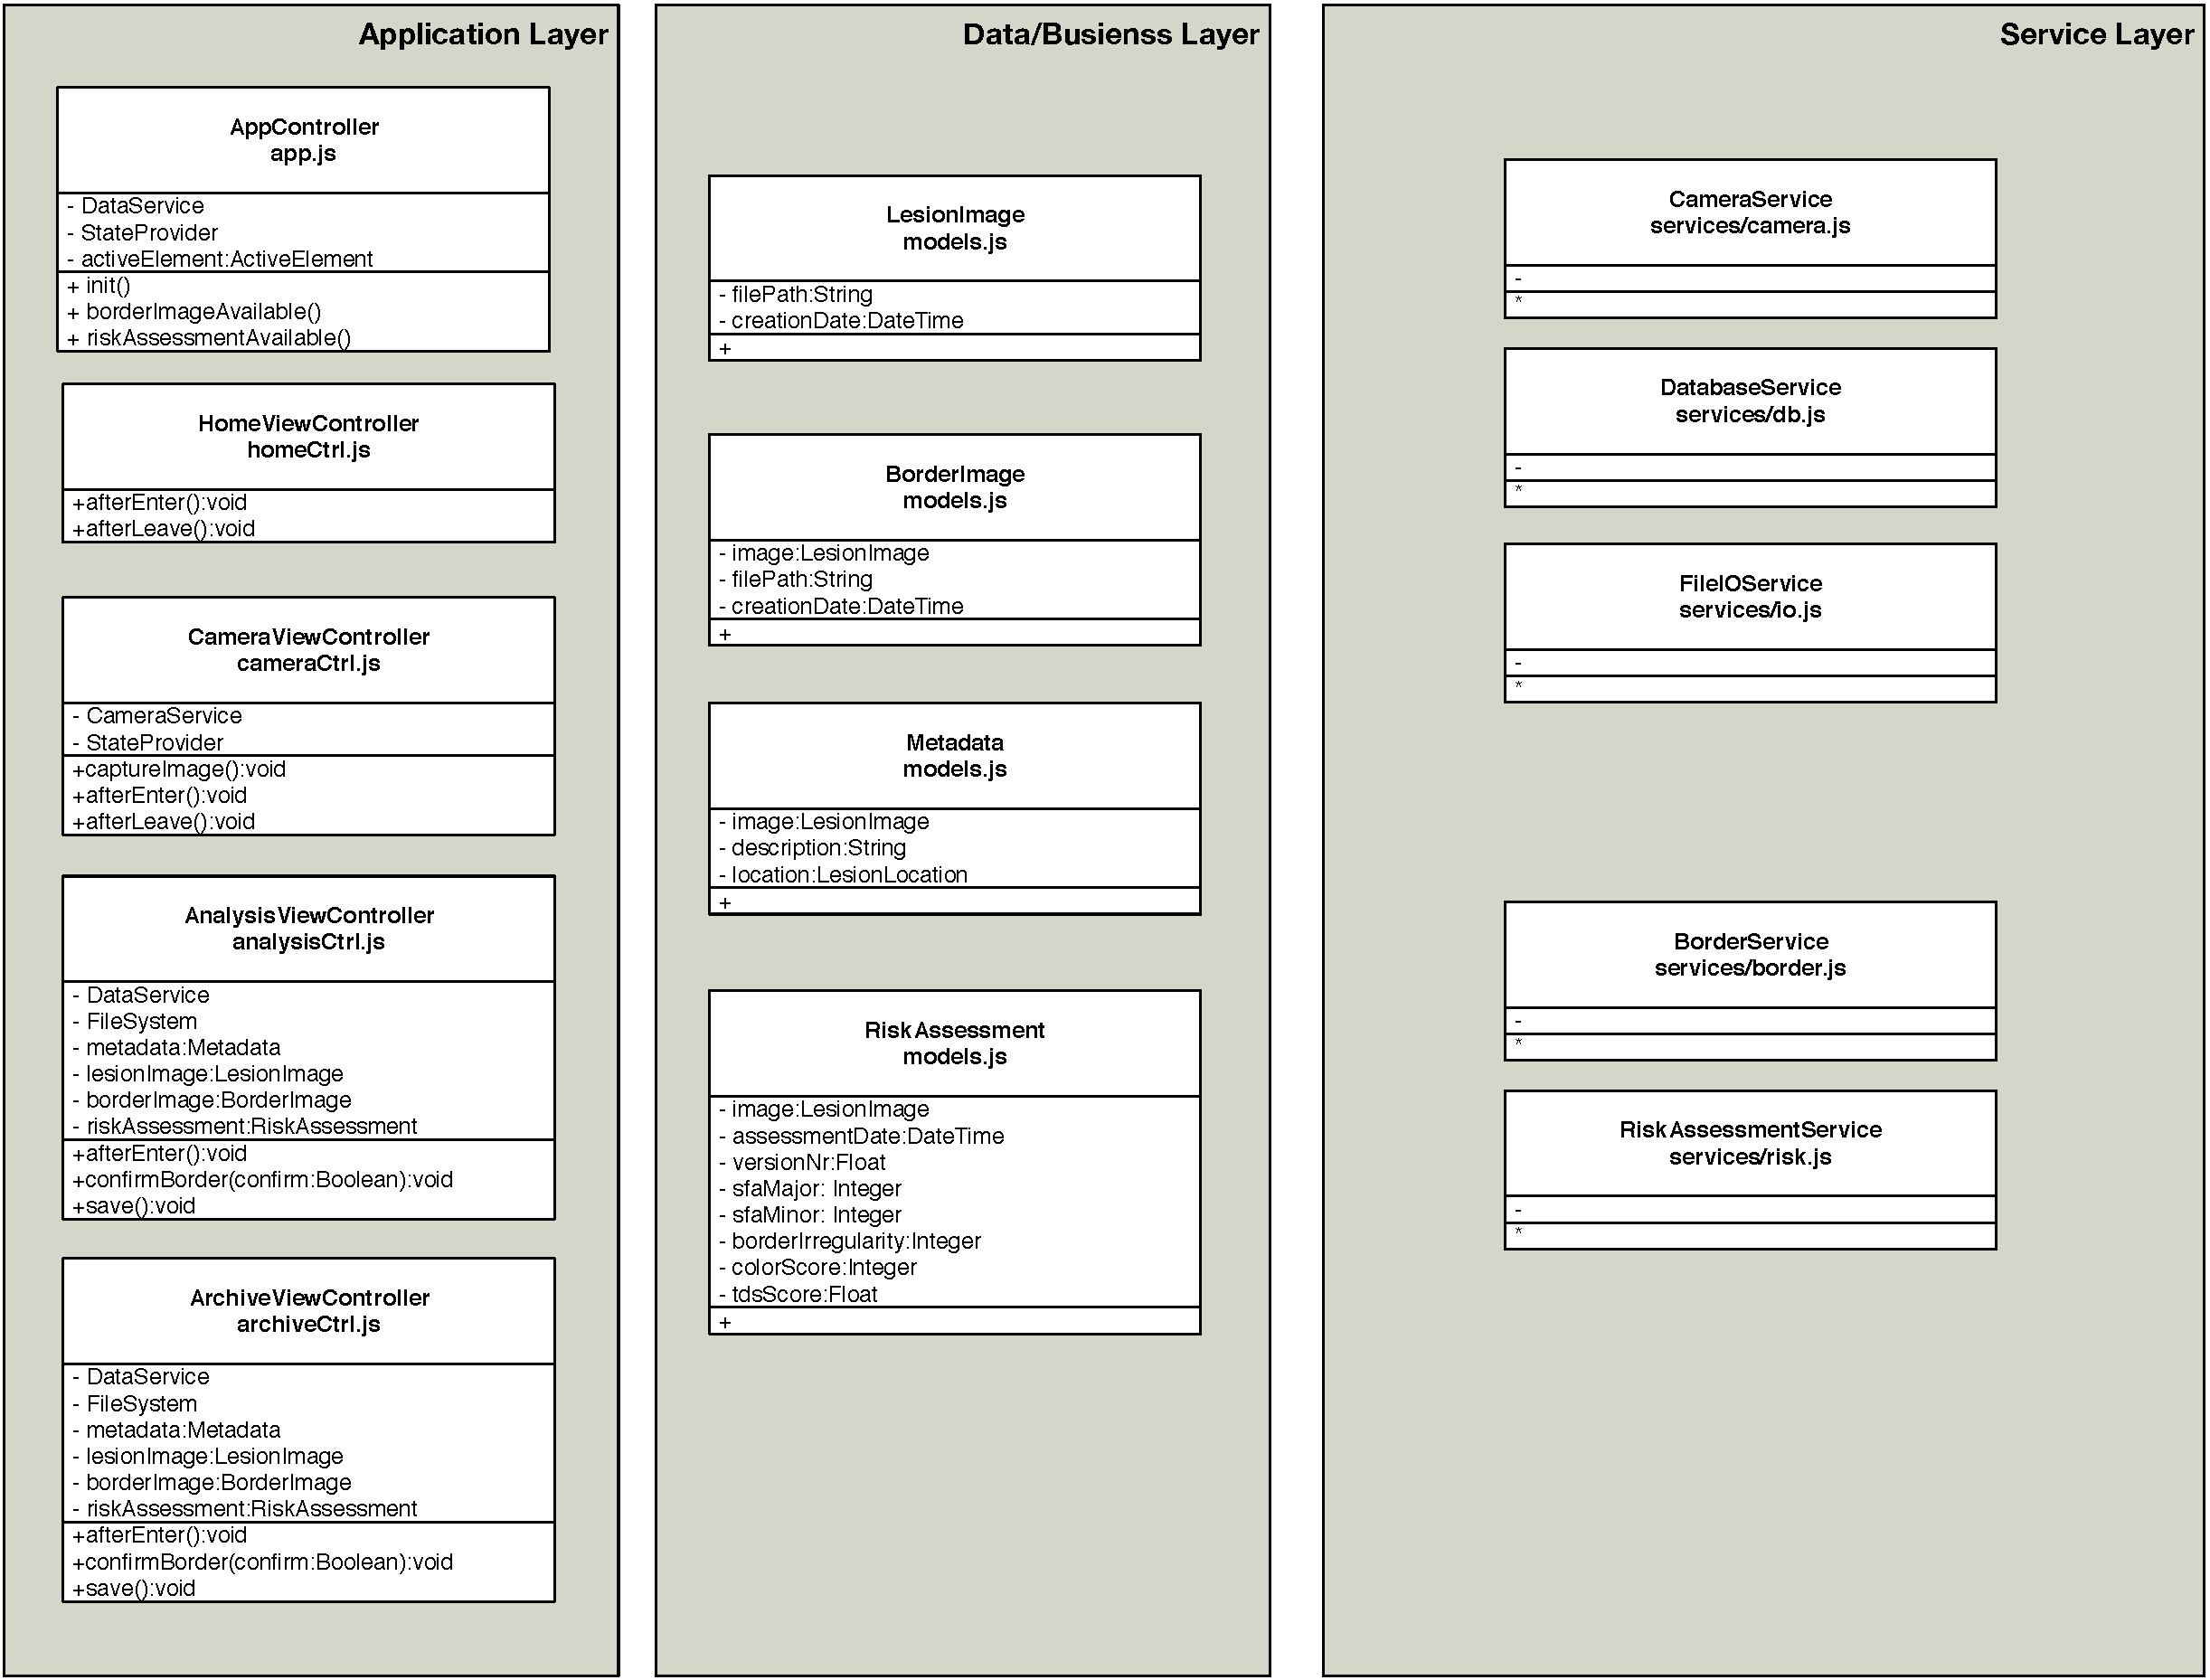
\includegraphics[width=\textwidth,keepaspectratio]{assets/architecture/class_diagram.pdf}
    \caption{Component diagram of the MDApp}
    \label{fig:class_dia}
\end{figure}

    \subsubsection{Application Layer}
        \paragraph{AppController}
                            \begin{longtable}[H]{  | >{\bfseries}l | l | l | l | l | }

                    \hline

                    Name
                    & \multicolumn{4}{l |}{AppController} \\ \hline

                    Description
                    & \multicolumn{4}{p{8.5cm} |}{The AppController manages the global state of the app. It can disable UI elements when the app needs to wait for longer processes. It can restore the previous state of the app after it has been reopened or updated.} \\ \hline

                    Type
                    & \multicolumn{4}{l |}{Class}
                    \\ \hline

                    Implemented In
                    & \multicolumn{4}{l |}{app.js}
                    \\ \hline

                    Attributes
                    & Name & Type & \multicolumn{2}{p{6.5cm} |}{Description} \\ \hline
                        & \$state & class & \multicolumn{2}{p{6.5cm} |}{
                        The \$state object is provided by the angular ui-router and is used to define pages in the app. It can be used to query or set the ui state. The AppController uses the \$state to automatically move the user from the camera view to the analysis view when the border data has become available, for example.
                        } \\ \hline
                        & MDAppState & class & \multicolumn{2}{p{6.5cm} |}{
                        The MDAppState stores data the the AppController might need to restore it's state after a restart.
                        } \\ \hline
                        & uiDisabled & boolean & \multicolumn{2}{p{6.5cm} |}{
                        This variable is used to trigger changes in the ui. Through 2-way binding the ui components in the view will become disabled or enabled respectivly.
                        } \\ \hline
                        & tabStates & object & \multicolumn{2}{p{6.5cm} |}{
                        This javascript object stored the disabled-state of the individual tab components in the ui. The AppController disabiles or enables specific tab elements based on the state of the app and the data currently available.
                        } \\ \hline


                    Methods
                    & Name & Parameter & Return Type & Description \\ \hline

                        &


                \end{longtable}


